\documentclass[aspectratio=169,10pt]{beamer}
\usetheme[progressbar=frametitle,numbering=fraction]{metropolis}
\usepackage[utf8]{inputenc}
\usepackage[T1]{fontenc}
\usepackage[brazil]{babel}
\usepackage{booktabs}
\usepackage{graphicx}
\usepackage{xcolor}
\graphicspath{{../figures/}}

% paleta preto, branco e amarelo
\definecolor{preto}{HTML}{111111}
\definecolor{amarelo}{HTML}{FFC300}
\definecolor{ouro}{HTML}{9E7700}   % amarelo escuro para texto (legível sobre branco)
\definecolor{cinza}{HTML}{52514e}
\definecolor{cinzaclaro}{HTML}{3a3a3a}
\setbeamercolor{normal text}{fg=preto,bg=white}
\setbeamercolor{frametitle}{fg=white,bg=preto}
\setbeamercolor{structure}{fg=preto}
\setbeamercolor{alerted text}{fg=ouro}
\setbeamerfont{alerted text}{series=\bfseries}
\setbeamercolor{progress bar}{fg=amarelo,bg=cinzaclaro}
\setbeamercolor{title separator}{fg=amarelo}
\setbeamercolor{page number in head/foot}{fg=cinza}
\setbeamercolor{item projected}{fg=preto}
\setbeamertemplate{itemize item}{\color{amarelo}\textbullet}
\setbeamertemplate{itemize subitem}{\color{amarelo}\textbullet}
\setbeamerfont{footnote}{size=\tiny}
\newcommand{\fonte}[1]{\par\vfill{\tiny\color{cinza}#1}}

\title{O preço de um hack}
\subtitle{Como o mercado de criptoativos reage a falhas de segurança em blockchain}
\author{Equipe Os D: Yoonsik Hur, Carolina Thomaz Ferreira Curraladas, Miguel Absy Freire de Oliveira,\\ Murilo Santos de Castro e Gustavo Katsuo Tsutsui}
\institute{7º Desafio de Dados de Moedas Digitais FGV \textbullet{} FGV EESP Digital Finance \textbullet{} Ripple UBRI}
\date{Novembro de 2026}

\begin{document}

% ---------------------------------------------------------------- 1
\begin{frame}[plain]
\vspace{0.6cm}
{\LARGE\bfseries O preço de um hack}\\[4pt]
{\large Como o mercado de criptoativos reage a falhas de segurança em blockchain}\\[2pt]
{\color{amarelo}\rule{\textwidth}{2pt}}

\vspace{0.4cm}
\begin{columns}[T]
\begin{column}{0.62\textwidth}
\normalsize
\alert{2026 é o ano recorde de exploits}: 333 incidentes até 06/11 (217 em 2024) e US\$ 8{,}8 bi em perdas, dos quais US\$ 6,4 bi em um só evento (Binance, outubro).

\medskip
A tokenização de ativos depende de que essa infraestrutura seja segura.

\medskip
\textbf{Quanto um hack custa a quem detém criptoativos, além do valor roubado?}
\end{column}
\begin{column}{0.34\textwidth}
\small\color{cinza}
\textbf{Equipe Os D}\\
Yoonsik Hur\\
Carolina Thomaz Ferreira Curraladas\\
Miguel Absy Freire de Oliveira\\
Murilo Santos de Castro\\
Gustavo Katsuo Tsutsui
\end{column}
\end{columns}

\vfill
{\scriptsize\color{cinza}7º Desafio de Dados de Moedas Digitais FGV \textbullet{} FGV EESP Digital Finance \textbullet{} Ripple UBRI \textbullet{} Novembro de 2026}
\end{frame}

% ---------------------------------------------------------------- 2
\begin{frame}[t]{Pergunta, tese e hipóteses}
\small
\textbf{Pergunta.} Como o mercado precifica uma falha de segurança: no token do protocolo, nos depósitos, na própria blockchain e nos protocolos que dependem do mesmo código?

\smallskip
\textbf{Tese.} A segurança da infraestrutura é um determinante do valor das moedas digitais e uma condição para a tokenização.

\smallskip
\textbf{Hipóteses}, registradas no repositório antes de cada resultado (qualquer resultado é reportado):
\begin{enumerate}\footnotesize\setlength{\itemsep}{0pt}
\item[H1] Exploits geram retorno anormal negativo no token e corrida bancária on-chain além do valor roubado.
\item[H2] Falhas operacionais e de governança são punidas mais que bugs de código, dado o tamanho da perda (sinalização).
\item[H3] Auditoria prévia e devolução dos fundos atenuam a reação.
\item[H4] Exploits grandes afetam a moeda nativa da chain, provocam migração para stablecoins e quebram a paridade de ativos wrapped.
\item[H5] Protocolos com dependência técnica da vítima (fork do mesmo código) sofrem contágio, semelhantes sem a dependência não.
\end{enumerate}

\smallskip
\textbf{Resposta curta.} H1 e H4 (moeda nativa) confirmadas. H2, H3 e H5 não. \alert{O dano de um hack é grande, rápido e local}.
\end{frame}

% ---------------------------------------------------------------- 3
\begin{frame}{Dados e taxonomia de falhas}
\begin{columns}[T]
\begin{column}{0.44\textwidth}
\small
\textbf{Fontes públicas (DefiLlama).} Hacks, 8.966 protocolos, TVL diário por token, preços de 412 moedas, stablecoins e TVL de 100 chains.

\medskip
\textbf{Amostra.} 1.341 incidentes $\rightarrow$ \textbf{581} de 2020 em diante com perda $\geq$ US\$ 1 mi (3 duplicatas removidas) $\rightarrow$ 132 com preço do token e 125 com TVL por token em toda a janela.

\medskip
\textbf{Validação manual.} Datas dos 35 maiores eventos em fontes externas, 5 reclassificações justificadas e devolução de fundos recodificada.
\end{column}
\begin{column}{0.54\textwidth}
\scriptsize
\textbf{Taxonomia pelo mecanismo do ataque} (81 técnicas $\rightarrow$ 6 categorias)\\[2pt]
\begin{tabular}{@{}lrrrr@{}}
\toprule
Categoria & Eventos & Perda (US\$ bi) & Preço & TVL\\
\midrule
Lógica de contrato & 240 & 3,9 & 73 & 58\\
Chave ou infraestrutura & 196 & 18,2 & 30 & 26\\
Oráculo ou preço & 73 & 0,9 & 23 & 34\\
Bridge cross-chain & 32 & 1,5 & 6 & 6\\
Governança & 13 & 0,3 & 2 & 2\\
Outros (inclui rugpull) & 27 & 0,4 & 0 & 1\\
\midrule
\textbf{Total} & \textbf{581} & \textbf{25,1} & \textbf{134} & \textbf{127}\\
\bottomrule
\end{tabular}

\medskip
Para H2: \emph{operacional} (chave, infraestrutura, governança) contra \emph{código} (contrato, bridge). Ser bridge é uma dummy à parte, para não confundir H2 com H4.
\end{column}
\end{columns}
\fonte{Fonte: api.llama.fi, coins.llama.fi e stablecoins.llama.fi, coletados em 08/11/2026.}
\end{frame}

% ---------------------------------------------------------------- 4
\begin{frame}{Metodologia}
\small
\begin{columns}[T]
\begin{column}{0.5\textwidth}
\textbf{Estudo de evento (H1)}
\begin{itemize}\small
\item Dias corridos (mercado 24/7). Modelo de mercado em [$-120$, $-11$] com ETH. Robustez com moeda nativa e índice DeFi equal-weighted fixado antes.
\item CAR e BHAR em [$-1$,$+1$] a [0,$+30$]. Testes BMP, Corrado, bootstrap e Wilcoxon.
\item \textbf{TVL decomposto token a token} em efeito preço e fluxo líquido. Corrida = fluxo anormal \emph{descontado o valor roubado}.
\end{itemize}
\textbf{Corte transversal (H2, H3)}
\begin{itemize}\small
\item MQO com erros HC3: tipo de falha, log da perda, auditoria, devolução, bridge, ciclo de mercado e efeitos fixos de chain.
\end{itemize}
\end{column}
\begin{column}{0.5\textwidth}
\textbf{Nível da blockchain (H4)}
\begin{itemize}\small
\item Perda relativa ao TVL da chain. Retorno anormal da moeda nativa (benchmark BTC), crescimento anormal de stablecoins e paridade de wrapped.
\end{itemize}
\textbf{Contágio (H5)}
\begin{itemize}\small
\item Rede de forks. \textbf{Diferenças em diferenças}: forks da vítima contra protocolos da mesma categoria e chain, com efeito fixo de evento.
\end{itemize}
\textbf{Robustez}
\begin{itemize}\small
\item Placebo com 1.000 conjuntos de datas sem hack, datas originais da fonte, sem eventos sobrepostos, sem crises (Terra, FTX, outubro de 2025 e de 2026), outros cortes de perda.
\end{itemize}
\end{column}
\end{columns}
\end{frame}

% ---------------------------------------------------------------- 5
\begin{frame}{H1: o token cai 17\% no dia, e os depósitos saem aos poucos}
\begin{columns}[T]
\begin{column}{0.5\textwidth}
\centering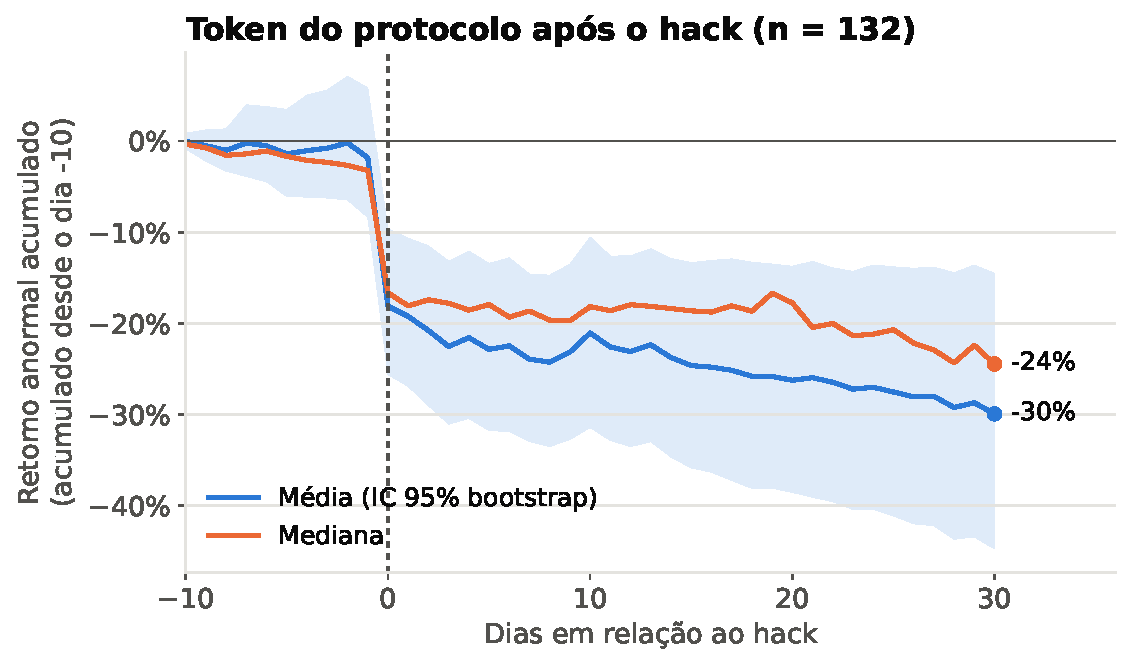
\includegraphics[width=\linewidth,height=0.5\textheight,keepaspectratio]{fig3_price_car_path.pdf}
\end{column}
\begin{column}{0.5\textwidth}
\centering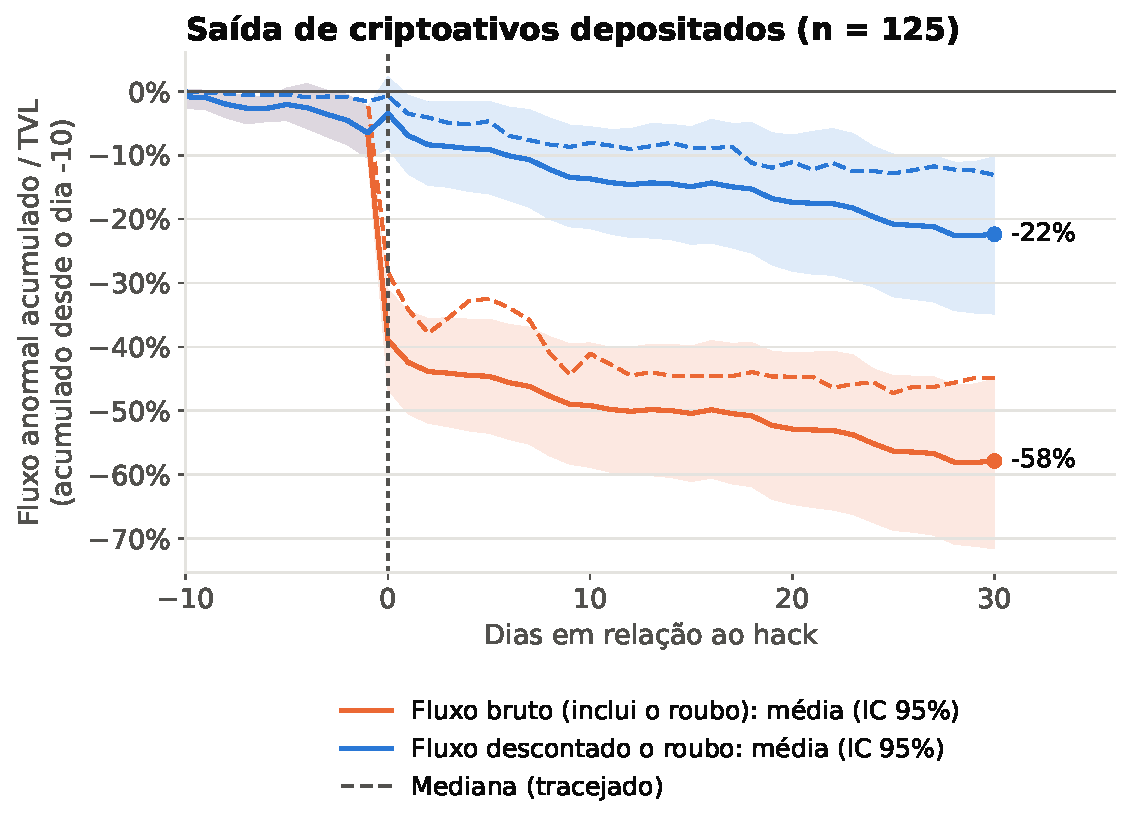
\includegraphics[width=\linewidth,height=0.5\textheight,keepaspectratio]{fig3_tvl_flow_path.pdf}
\end{column}
\end{columns}
\small
\begin{itemize}
\item \textbf{Preço}: CAR[0,$+1$] de \alert{$-17$\%} (mediana $-14$\%, 87\% dos eventos negativos). Placebo entre $-2$\% e $+3$\%. Em 30 dias, mediana de $-19$\%.
\item \textbf{Depósitos}: saída bruta de 36\% do TVL em dois dias, quase toda o próprio roubo. Descontados o roubo e a deriva do placebo, a \alert{corrida extra é de cerca de 10\% do TVL em 30 dias} (p = 0,01).
\end{itemize}
\end{frame}

% ---------------------------------------------------------------- 6
\begin{frame}{H2 e H3: o tipo de falha não muda o castigo de forma detectável}
\begin{columns}[T]
\begin{column}{0.56\textwidth}
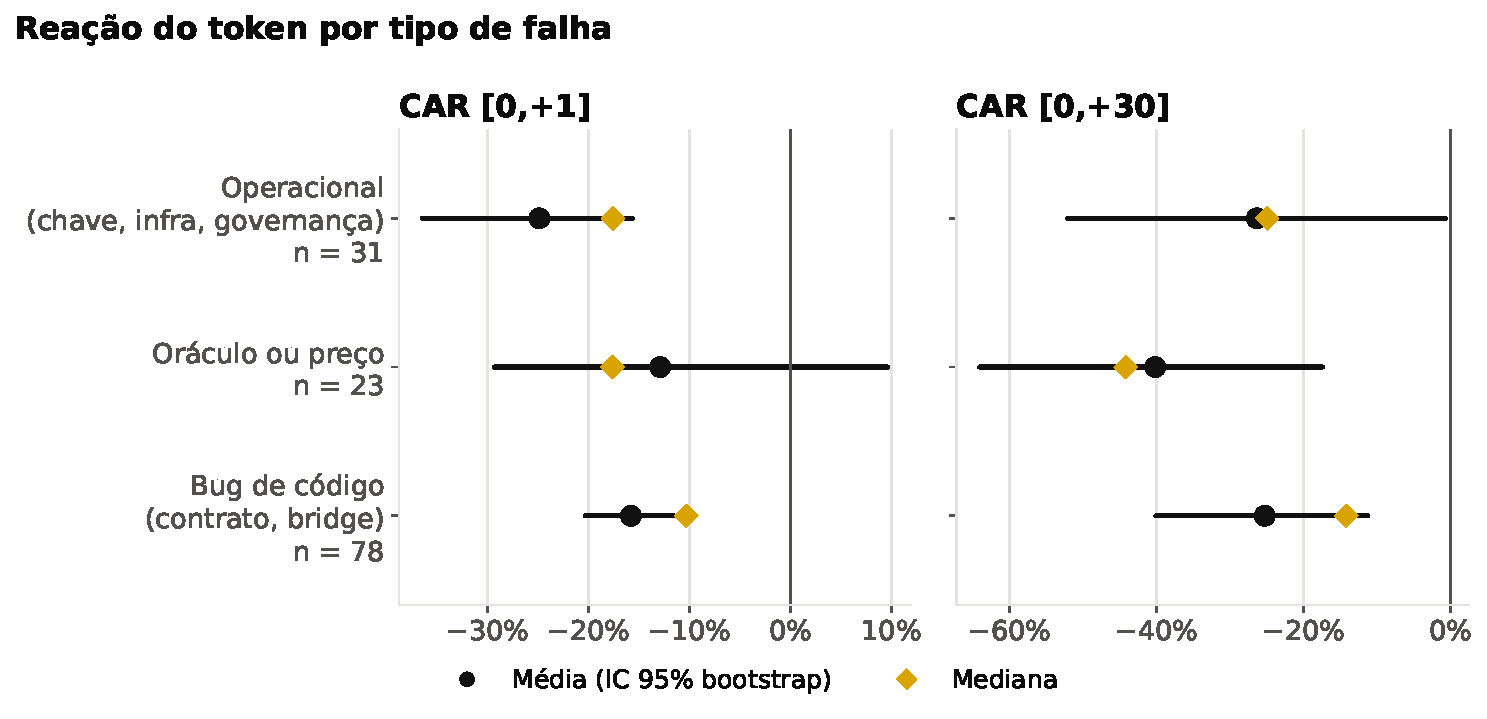
\includegraphics[width=\linewidth]{fig4_car_by_failure_type.pdf}
\end{column}
\begin{column}{0.44\textwidth}
\small
\begin{itemize}
\item Falhas operacionais caem mais no dia ($-25$\% contra $-16$\% de bugs de código), na direção de H2.
\item Com controles a diferença é de $-7$ p.p., com IC 95\% de $-19$ a $+5$ p.p. O efeito mínimo detectável é de 17 p.p. \alert{Descartamos uma punição extra maior que cerca de 19 p.p.}, não diferenças menores.
\item \textbf{O que explica a reação é o tamanho}: cada log de perda a mais reduz o CAR de 30 dias em 8 p.p. (p = 0,03).
\item H3: auditoria e devolução sem efeito em nenhuma especificação (só 9 devoluções, auditoria medida hoje).
\end{itemize}
\end{column}
\end{columns}
\end{frame}

% ---------------------------------------------------------------- 7
\begin{frame}{H4 e H5: a chain sente hacks grandes, os forks não sentem nada}
\begin{columns}[T]
\begin{column}{0.62\textwidth}
\centering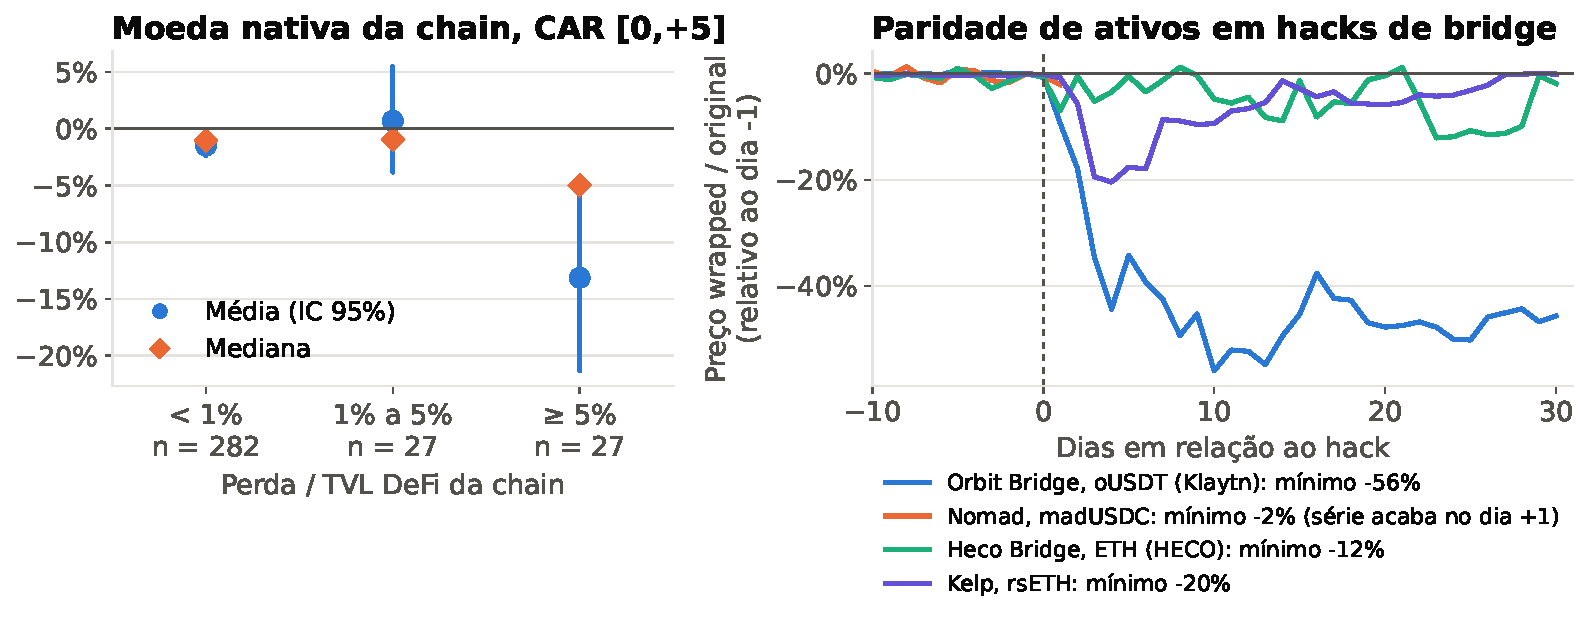
\includegraphics[width=\linewidth,height=0.5\textheight,keepaspectratio]{fig5_chain_level.pdf}
\end{column}
\begin{column}{0.38\textwidth}
\centering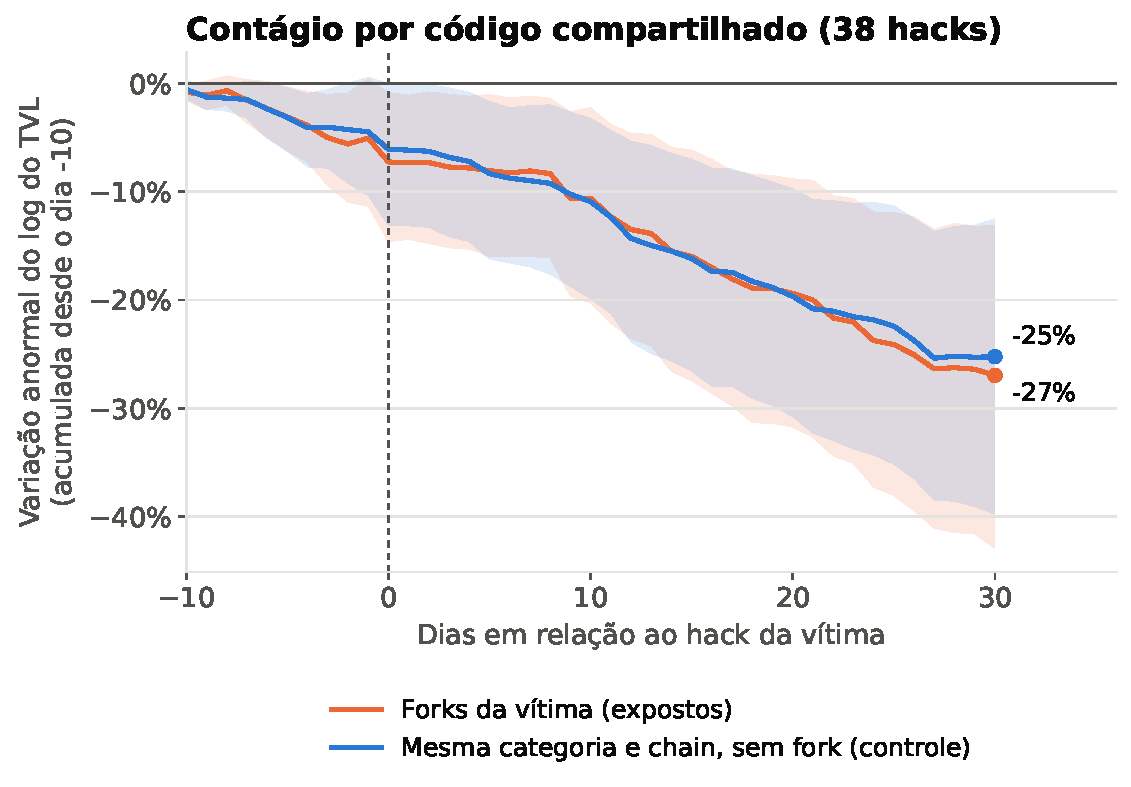
\includegraphics[width=\linewidth,height=0.5\textheight,keepaspectratio]{fig6_fork_contagion.pdf}
\end{column}
\end{columns}
\scriptsize
\begin{itemize}
\item \textbf{Moeda nativa}: com perda $\geq$ 5\% do TVL da chain (n = 27), \alert{$-7{,}5$\% em [0,$+1$] e $-13$\% em [0,$+5$]}, com dose-resposta significativa.
\item \textbf{Stablecoins}: ao contrário de H4, a oferta na chain \emph{cai} ($-6$\% em 30 dias). O capital sai da rede, não se refugia nela. \textbf{Wrapped}: o oUSDT da Orbit perdeu 56\% da paridade.
\item \textbf{Contágio por fork (38 hacks, 315 protocolos)}: efeito de $+0{,}3$ p.p. em [0,$+1$], IC de $-2{,}0$ a $+2{,}6$ p.p. Sem contágio pelo código copiado. Sinal fraco de contágio setorial ($-5{,}5$ p.p. sobre o placebo, p = 0,04).
\end{itemize}
\end{frame}

% ---------------------------------------------------------------- 8
\begin{frame}{Robustez e limitações}
\begin{columns}[T]
\begin{column}{0.58\textwidth}
\centering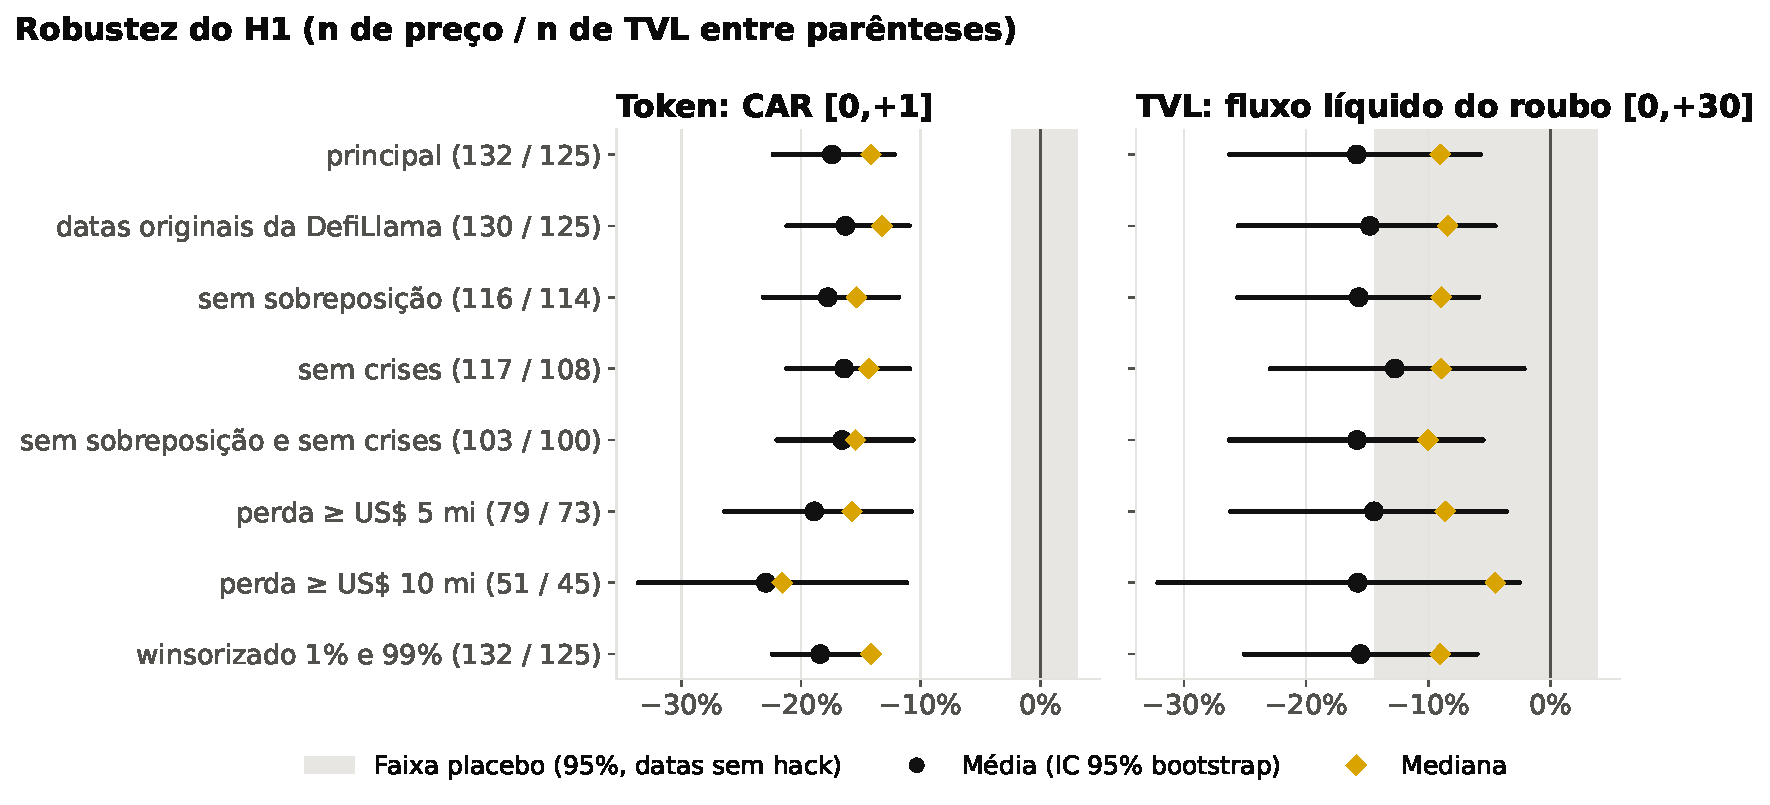
\includegraphics[width=\linewidth]{fig7_robustness.pdf}
\end{column}
\begin{column}{0.42\textwidth}
\scriptsize
\textbf{O que resiste}: a queda do dia do hack, em todas as variações e no placebo.

\smallskip
\textbf{O que o placebo ensinou}: a média do CAR de 30 dias não serve de prova (placebo de $-26$\% a $+82$\%), então usamos mediana e log-CAR. O TVL cai 6\% em 30 dias mesmo sem hack, e isso já foi descontado.

\smallskip
\textbf{Limitações}
\begin{itemize}\scriptsize
\item Sem volume na fonte gratuita, logo sem filtro de liquidez.
\item Auditoria medida hoje, não na data do hack.
\item Só 4 bridges com preço do wrapped.
\item Erros de fuso de um dia nas datas da fonte.
\item H2 e H3 com pouco poder (31 eventos operacionais, 9 devoluções).
\end{itemize}
\end{column}
\end{columns}
\end{frame}

% ---------------------------------------------------------------- 9
\begin{frame}{Onde está o risco hoje: concentração em um protocolo por chain}
\begin{columns}[T]
\begin{column}{0.6\textwidth}
\centering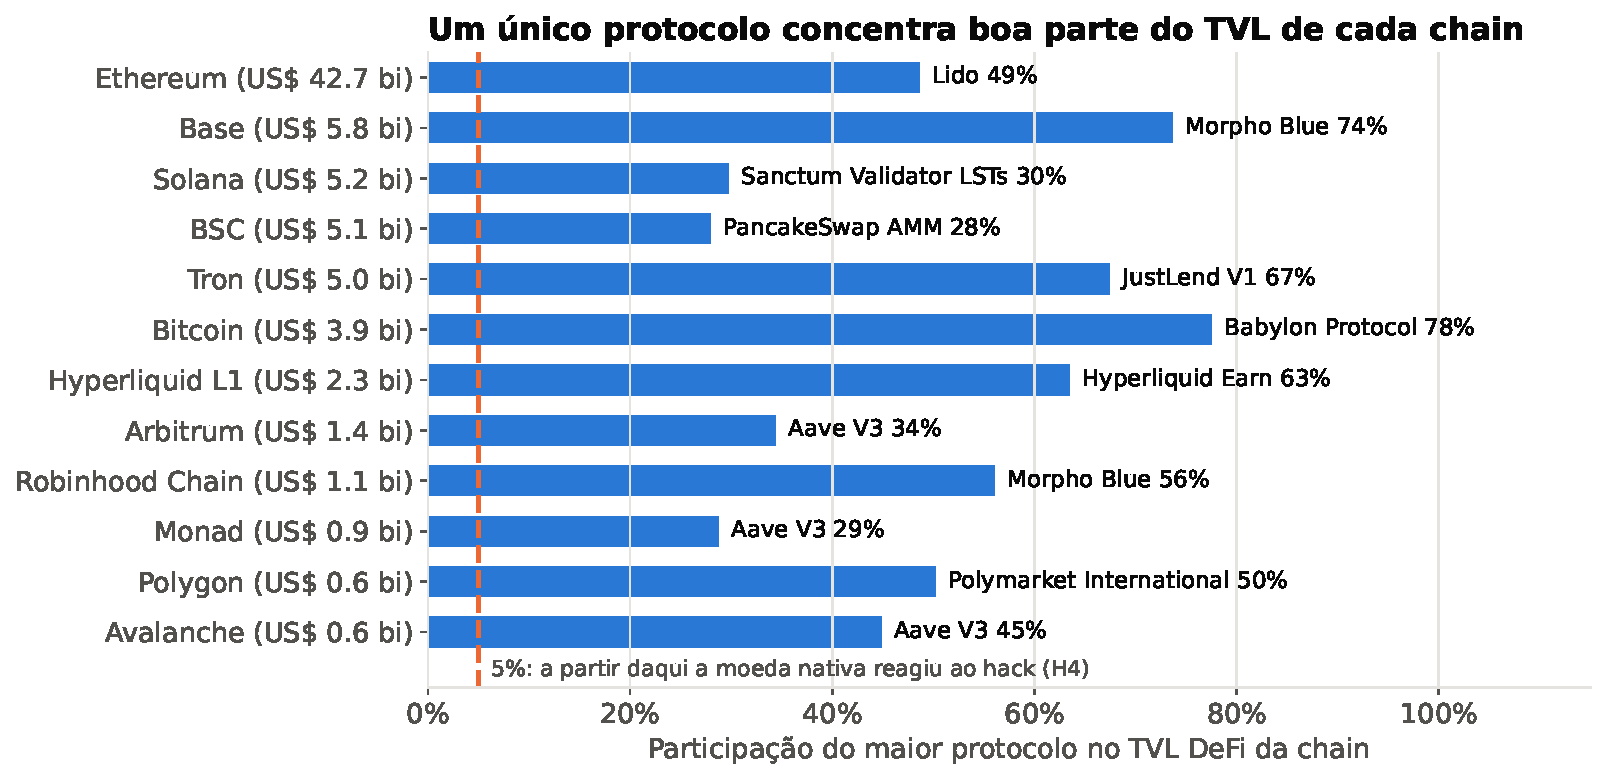
\includegraphics[width=\linewidth,height=0.72\textheight,keepaspectratio]{fig8_chain_concentration.pdf}\\[-2pt]{\tiny\color{cinza}Fotografia de 08/11/2026. TVL DeFi oficial por chain, sem CEX e bridges.}
\end{column}
\begin{column}{0.4\textwidth}
\small
\begin{itemize}
\item \textbf{171 protocolos} passam de 5\% do TVL de alguma chain. Nas 12 maiores chains, o maior protocolo tem de 28\% a 78\%.
\item Um hack de um terço do Lido ou do Morpho Blue na Base já teria a escala em que a moeda nativa reagiu (H4).
\item \textbf{Morpho Blue} (17 chains) e \textbf{Aave V3} (15) são pontos únicos de falha em várias redes.
\end{itemize}
\scriptsize\color{cinza} O limiar vem de chains com TVL mediano de US\$ 114 mi. No Ethereum é extrapolação.
\end{column}
\end{columns}

\end{frame}

% ---------------------------------------------------------------- 10
\begin{frame}{Implicações: o que aprendemos e por que importa}
\small
\begin{columns}[T]
\begin{column}{0.5\textwidth}
\textbf{Investidores.} Um hack custa cerca de 17\% do token no dia, proporcional ao tamanho da perda, e fica na vítima. Diversificar entre protocolos funciona, mesmo entre forks do mesmo código.

\medskip
\textbf{Protocolos.} Não detectamos punição extra por tipo de falha: toda falha custa caro. A corrida de depósitos leva semanas, então a resposta nos primeiros dias importa.

\medskip
\textbf{Seguradoras on-chain.} A perda de um evento tem ordem de grandeza conhecida ($-17$\% no token, $-10$\% extra no TVL). Como não há contágio por fork, o risco entre protocolos é diversificável. O risco agregado está na concentração dentro de cada chain.
\end{column}
\begin{column}{0.5\textwidth}
\textbf{Reguladores e tokenização.} Grandes chains dependem de um único protocolo com 30\% a 80\% do TVL. Exigências de resiliência para esses pontos únicos de falha, e de transparência padronizada sobre incidentes (data, valor, devolução), são condição para a adoção institucional.

\medskip
\textbf{O que aprendemos}
\begin{itemize}\small
\item O mercado de moedas digitais precifica a segurança da infraestrutura, e rápido.
\item O dano é \alert{grande, rápido e local}: vítima e, em hacks grandes, a chain.
\item Rigor importa: o placebo mudou a leitura de 30 dias e os dados da fonte exigiram validação manual.
\end{itemize}
\end{column}
\end{columns}
\fonte{Código, dados e log de decisões disponíveis como material suplementar.}
\end{frame}

\end{document}
